 
 
\documentclass{beamer}
\usetheme{AnnArbor}
\usecolortheme{beaver}

\usepackage{wrapfig}
\usepackage{graphicx}
\usepackage{listings}
\usepackage{amsmath}
\usepackage{amssymb}
\usepackage{color}

\lstset{ %
  basicstyle=\footnotesize,           % the size of the fonts that are used for the code
  numbers=left,                   % where to put the line-numbers
  numberstyle=\tiny\color{gray},  % the style that is used for the line-numbers
  stepnumber=2,                   % the step between two line-numbers. If it's 1, each line 
                                  % will be numbered
  numbersep=5pt,                  % how far the line-numbers are from the code
  backgroundcolor=\color{white},      % choose the background color. You must add \usepackage{color}
  showspaces=false,               % show spaces adding particular underscores
  showstringspaces=false,         % underline spaces within strings
  showtabs=false,                 % show tabs within strings adding particular underscores
  frame=single,                   % adds a frame around the code
  rulecolor=\color{black},        % if not set, the frame-color may be changed on line-breaks within not-black text (e.g. commens (green here))
  tabsize=4,                      % sets default tabsize to 2 spaces
  captionpos=b,                   % sets the caption-position to bottom
  breaklines=true,                % sets automatic line breaking
  breakatwhitespace=false,        % sets if automatic breaks should only happen at whitespace
  keywordstyle=\color{blue},          % keyword style
  commentstyle=\color{dkgreen},       % comment style
  stringstyle=\color{mauve},         % string literal style
  escapeinside={\%*}{*)},            % if you want to add a comment within your code
  morekeywords={*,...}               % if you want to add more keywords to the set
}

\title
{libqcpp: A C++ quantum circuit simulator}
\subtitle{Architecture and Usage}
\author
{Steven Braeger}
\date{\today}

\input{Qcircuit}

\begin{document}
\frame{\titlepage} 


\begin{frame}
\frametitle{Table of Contents}
\tableofcontents
\end{frame}

\section{Theory}
\subsection{Quantum Register Machine Model}

\begin{frame}
  \frametitle{Quantum Register Model}
   \begin{itemize}
    \item Problem:  Simulate arbitrary quantum computations
    \item Simulation needs to be straightforward
    \item Express computations
    \item A good language and a good model go hand in hand!
   \end{itemize}
\end{frame}

\begin{frame}
   \frametitle{Quantum Turing Machine}

\begin{columns}[c]
\column{2.5in}
   \begin{itemize}
    \item define a unitary transition operator
    \item define a set of states
    \item define a quantum tape
    \item Not Easy to Program! (data structure)
    \item Not Easy to Simulate!(branching)
    \item Not Easy to Express! (language?)
   \end{itemize}
\column{2in}
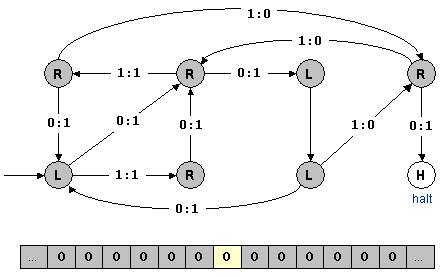
\includegraphics[width=\textwidth]{./beaverTM.png}
\end{columns}

\end{frame}

\begin{frame}
\frametitle{Quantum Circuits}
\begin{columns}[c]
\column{2.5in}
   \begin{itemize}
    \item define wires
    \item define gates
    \item Not Easy to Program! (data state?)
    \item Easy to Simulate! 
    \item Moderately Easy to Express (draw)
   \end{itemize}
\column{2in}
\Qcircuit @C=1em @R=.7em {
& \ctrl{2} & \targ & \gate{U} & \qw \\
& \qw & \ctrl{-1} & \qw & \qw \\
& \targ & \ctrl{-1} & \ctrl{-2} & \qw \\
}

\end{columns}

\end{frame}

\begin{frame}[fragile]
\frametitle{Quantum Register Machine}
\begin{columns}[c]
\column{2.5in}
   \begin{itemize}
    \item define operations
    \item define in sequence
    \item quantum state stored in register
    \item Easy to Program! (RM)
    \item Easy to Simulate! 
    \item Easy to Express (Register Program)
   \end{itemize}
\column{2in}
 \lstinputlisting[language=Plasm]{ramasm.s}

\end{columns}

\end{frame}

\begin{frame}[fragile]
\frametitle{Quantum Register Machine (cont.)}

\begin{columns}[r]
\column{2in}
 \Qcircuit @C=1em @R=.7em {
\lstick{q0} & \targ & \ctrl{2} & \targ & \gate{U} & \qw \\
\lstick{q1} & \qw & \qw & \ctrl{-1} & \qw & \qw \\
\lstick{q2} & \ctrl{-2} & \targ & \ctrl{-1} & \ctrl{-2} & \qw \\
}
\column{2in}
 \lstinputlisting[language=Plasm]{ramasm2.s}

\end{columns}

\begin{itemize}
 \item No branching
 \item No reading a quantum bit into a standard bit
 \item Can mix register machine 
 \item Equivalent to circuit model with save registers
\end{itemize}
\end{frame}
\subsection{Permutation Mechanics}

\begin{frame}
\frametitle{Matrix Mechanics}

Simple matrix mechanics for single gates

\begin{columns}[c]
\column{1.5in}
  \begin{equation*}
   \begin{bmatrix}
    1 & 0 & 0 & 0 \\ 
    0 & 1 & 0 & 0 \\
    0 & 0 & 0 & 1 \\
    0 & 0 & 1 & 0 
   \end{bmatrix}
    \begin{bmatrix} 
      \phi_{00} \\
      \phi_{01} \\
      \phi_{10}  \\
      \phi_{11} \\
    \end{bmatrix}
  \end{equation*}
\column{1.5in}
    \Qcircuit @C=1em @R=.7em {
\lstick{q0} & \targ &  \qw \\
\lstick{q1} & \ctrl{-1}& \qw \\
}
\end{columns}
\end{frame}

\begin{frame}
\frametitle{Matrix Mechanics}
 \begin{itemize}
  \item An operation on an $n$ bit register is a linear operation on the $2^n$ element quantum state vector $\ket{\phi}$
  \item Therefore, its a $2^n \times 2^n$ matrix operation.
  \item Transforms $\ket{\phi}$ into $\hat{\ket{\phi}}$
  \item $\hat{\ket{\phi}} = Mg \ket{\phi}$
 \end{itemize}
\end{frame}


\begin{frame}
 \frametitle{Matrix Mechanics}

What about multiple wires?

\begin{center}
\begin{minipage}{\paperwidth}
  \Qcircuit @C=2em @R=2em {
\lstick{q0} & \targ &  \qw \\
\lstick{q1} & \ctrl{-1} & \qw \\
\lstick{q2} & \qw &  \qw \\
\lstick{q3} & \qw & \qw \\
}
\end{minipage}
\end{center}
   

\end{frame}


\begin{frame}
\frametitle{Matrix Mechanics}

\begin{footnotesize}
  \begin{equation*}
   \left[\begin{array}{cccccccccccccccc}
   {\color{red}1} & {\color{red}0} & {\color{red}0} & {\color{red}0} & 0& 0& 0& 0& 0& 0& 0& 0& 0& 0& 0& 0\\ 
   {\color{red}0} & {\color{red}1} & {\color{red}0} & {\color{red}0} & 0& 0& 0& 0& 0& 0& 0& 0& 0& 0& 0& 0 \\
   {\color{red}0} & {\color{red}0} & {\color{red}0} & {\color{red}1} & 0& 0& 0& 0& 0& 0& 0& 0& 0& 0& 0& 0 \\
   {\color{red}0} & {\color{red}0} & {\color{red}1} & {\color{red}0} & 0& 0& 0& 0& 0& 0& 0& 0& 0& 0& 0& 0 \\
   0& 0& 0& 0& {\color{red}1} & {\color{red}0} & {\color{red}0} & {\color{red}0} & 0& 0& 0& 0& 0& 0& 0& 0\\ 
   0& 0& 0& 0& {\color{red}0} & {\color{red}1} & {\color{red}0} & {\color{red}0} & 0& 0& 0& 0& 0& 0& 0& 0 \\
   0& 0& 0& 0& {\color{red}0} & {\color{red}0} & {\color{red}0} & {\color{red}1} & 0& 0& 0& 0& 0& 0& 0& 0 \\
   0& 0& 0& 0& {\color{red}0} & {\color{red}0} & {\color{red}1} & {\color{red}0} & 0& 0& 0& 0& 0& 0& 0& 0 \\
   0& 0& 0& 0& 0& 0& 0& 0& {\color{red}1} & {\color{red}0} & {\color{red}0} & {\color{red}0}& 0& 0& 0& 0 \\ 
   0& 0& 0& 0& 0& 0& 0& 0& {\color{red}0} & {\color{red}1} & {\color{red}0} & {\color{red}0}& 0& 0& 0& 0 \\
   0& 0& 0& 0& 0& 0& 0& 0& {\color{red}0} & {\color{red}0} & {\color{red}0} & {\color{red}1}& 0& 0& 0& 0 \\
   0& 0& 0& 0& 0& 0& 0& 0& {\color{red}0} & {\color{red}0} & {\color{red}1} & {\color{red}0}& 0& 0& 0& 0 \\
   0& 0& 0& 0& 0& 0& 0& 0& 0& 0& 0& 0& {\color{red}1} & {\color{red}0} & {\color{red}0} & {\color{red}0} \\ 
   0& 0& 0& 0& 0& 0& 0& 0& 0& 0& 0& 0& {\color{red}0} & {\color{red}1} & {\color{red}0} & {\color{red}0} \\
   0& 0& 0& 0& 0& 0& 0& 0& 0& 0& 0& 0& {\color{red}0} & {\color{red}0} & {\color{red}0} & {\color{red}1} \\
   0& 0& 0& 0& 0& 0& 0& 0& 0& 0& 0& 0& {\color{red}0} & {\color{red}0} & {\color{red}1} & {\color{red}0} \\
   \end{array}\right]
    \begin{bmatrix} 
      \phi_{0000} \\
      \phi_{0001} \\
      \phi_{0010}  \\
      \phi_{0011} \\
      \phi_{0100} \\
      \phi_{0101} \\
      \phi_{0110}  \\
      \phi_{0111} \\
      \phi_{1000} \\
      \phi_{1001} \\
      \phi_{1010}  \\
      \phi_{1011} \\
      \phi_{1100} \\
      \phi_{1101} \\
      \phi_{1110}  \\
      \phi_{1111} \\
    \end{bmatrix}
  \end{equation*}
\end{footnotesize}


\end{frame}
 
\begin{frame}
 \frametitle{Matrix Permutations}

\begin{itemize}
 \item Application of a $k$-bit gate to the lower $k$-bits of an $m$-bit gate requires $2^m / 2^k$ block-diagonal applications of the $k$-bit gate.
 \item What about applying the gate to an arbitrary subset of the bits?
\end{itemize}

\begin{center}
\begin{minipage}{\paperwidth}
  \Qcircuit @C=2em @R=2em {
\lstick{q0} & \qw &  \qw \\
\lstick{q1} & \targ & \qw \\
\lstick{q2} & \qw &  \qw \\
\lstick{q3} & \ctrl{-2} & \qw \\
}
\end{minipage}
\end{center}

\begin{enumerate}
 \item Gate Matrix per permutation of input bits
 \item Permute desired bits to lower order bits, apply gate, permute back up
\end{enumerate}

   

\end{frame}

\begin{frame}
 \frametitle{Block-Matrix Diagonalization}

``cnot \$q3 \$q1''
\begin{footnotesize}
\begin{equation}
        \begin{bmatrix} 
      \phi_{{\color{blue}0}0{\color{cyan}0}0} \\
      \phi_{{\color{blue}0}0{\color{cyan}0}1} \\
      \phi_{{\color{blue}0}0{\color{cyan}1}0}  \\
      \phi_{{\color{blue}0}0{\color{cyan}1}1} \\
      \phi_{{\color{blue}0}1{\color{cyan}0}0} \\
      \phi_{{\color{blue}0}1{\color{cyan}0}1} \\
      \phi_{{\color{blue}0}1{\color{cyan}1}0}  \\
      \phi_{{\color{blue}0}1{\color{cyan}1}1} \\
      \phi_{{\color{blue}1}0{\color{cyan}0}0} \\
      \phi_{{\color{blue}1}0{\color{cyan}0}1} \\
      \phi_{{\color{blue}1}0{\color{cyan}1}0}  \\
      \phi_{{\color{blue}1}0{\color{cyan}1}1} \\
      \phi_{{\color{blue}1}1{\color{cyan}0}0} \\
      \phi_{{\color{blue}1}1{\color{cyan}0}1} \\
      \phi_{{\color{blue}1}1{\color{cyan}1}0}  \\
      \phi_{{\color{blue}1}1{\color{cyan}1}1} \\
    \end{bmatrix} 
  \longrightarrow
     \begin{bmatrix} 
      \phi_{00{\color{blue}0}{\color{cyan}0}} \\
      \phi_{00{\color{blue}0}{\color{cyan}1}} \\
      \phi_{00{\color{blue}1}{\color{cyan}0}}  \\
      \phi_{00{\color{blue}1}{\color{cyan}1}} \\
      \phi_{01{\color{blue}0}{\color{cyan}0}} \\
      \phi_{01{\color{blue}0}{\color{cyan}1}} \\
      \phi_{01{\color{blue}1}{\color{cyan}0}}  \\
      \phi_{01{\color{blue}1}{\color{cyan}1}} \\
      \phi_{10{\color{blue}0}{\color{cyan}0}} \\
      \phi_{10{\color{blue}0}{\color{cyan}1}} \\
      \phi_{10{\color{blue}1}{\color{cyan}0}}  \\
      \phi_{10{\color{blue}1}{\color{cyan}1}} \\
      \phi_{11{\color{blue}0}{\color{cyan}0}} \\
      \phi_{11{\color{blue}0}{\color{cyan}1}} \\
      \phi_{11{\color{blue}1}{\color{cyan}0}}  \\
      \phi_{11{\color{blue}1}{\color{cyan}1}} \\
    \end{bmatrix} 
\longrightarrow 
     \text{Apply gate to lower part}
\longrightarrow
     \begin{bmatrix} 
      \phi_{00{\color{blue}0}{\color{cyan}0}} \\
      \phi_{00{\color{blue}0}{\color{cyan}1}} \\
      \phi_{00{\color{blue}1}{\color{cyan}0}}  \\
      \phi_{00{\color{blue}1}{\color{cyan}1}} \\
      \phi_{01{\color{blue}0}{\color{cyan}0}} \\
      \phi_{01{\color{blue}0}{\color{cyan}1}} \\
      \phi_{01{\color{blue}1}{\color{cyan}0}}  \\
      \phi_{01{\color{blue}1}{\color{cyan}1}} \\
      \phi_{10{\color{blue}0}{\color{cyan}0}} \\
      \phi_{10{\color{blue}0}{\color{cyan}1}} \\
      \phi_{10{\color{blue}1}{\color{cyan}0}}  \\
      \phi_{10{\color{blue}1}{\color{cyan}1}} \\
      \phi_{11{\color{blue}0}{\color{cyan}0}} \\
      \phi_{11{\color{blue}0}{\color{cyan}1}} \\
      \phi_{11{\color{blue}1}{\color{cyan}0}}  \\
      \phi_{11{\color{blue}1}{\color{cyan}1}} \\
    \end{bmatrix} 
\longrightarrow
        \begin{bmatrix} 
      \phi_{{\color{blue}0}0{\color{cyan}0}0} \\
      \phi_{{\color{blue}0}0{\color{cyan}0}1} \\
      \phi_{{\color{blue}0}0{\color{cyan}1}0}  \\
      \phi_{{\color{blue}0}0{\color{cyan}1}1} \\
      \phi_{{\color{blue}0}1{\color{cyan}0}0} \\
      \phi_{{\color{blue}0}1{\color{cyan}0}1} \\
      \phi_{{\color{blue}0}1{\color{cyan}1}0}  \\
      \phi_{{\color{blue}0}1{\color{cyan}1}1} \\
      \phi_{{\color{blue}1}0{\color{cyan}0}0} \\
      \phi_{{\color{blue}1}0{\color{cyan}0}1} \\
      \phi_{{\color{blue}1}0{\color{cyan}1}0}  \\
      \phi_{{\color{blue}1}0{\color{cyan}1}1} \\
      \phi_{{\color{blue}1}1{\color{cyan}0}0} \\
      \phi_{{\color{blue}1}1{\color{cyan}0}1} \\
      \phi_{{\color{blue}1}1{\color{cyan}1}0}  \\
      \phi_{{\color{blue}1}1{\color{cyan}1}1} \\
    \end{bmatrix} 
\end{equation}
\end{footnotesize}

\end{frame}

\begin{frame}
 \frametitle{Permutation Algorithm}
 Mask: 000{\color{red}1}0{\color{red}11}00
 
 i: 000{\color{red}a}{\color{blue}x}{\color{red}bc}{\color{blue}yz}
 
 lindex: 000{\color{blue}xyz}{\color{red}abc}

 \lstinputlisting[basicstyle=\tiny,language=C++]{permute_down.cpp}

\end{frame}

\section{API}
\begin{frame}
  \frametitle{Simulation Architecture: API}
   
   \begin{itemize}
    \item Classes:  qgate
    \item qgate has an associated name and a number of gates $k$
    \item virtual apply() member function changes $2^k$ length state vector.
    \item state vector is std::vector\textless std::complex\textless double\textgreater \textgreater
   \end{itemize}

   \begin{itemize}
    \item class qram
    \item quantum register machine
    \item op() function takes a gate and a mask for which bits to apply it to.
   \end{itemize}

\end{frame}

\begin{frame}
 \frametitle{Circuit Example}

\begin{columns}[r]
\column{2in}
 \Qcircuit @C=1em @R=.7em {
\lstick{q0} & \qw & \targ & \targ & \gate{U} & \qw & \qw \\
\lstick{q1} & \targ & \qw & \ctrl{-1} & \qw & \qw & \meter \\
\lstick{q2} & \qw & \ctrl{-2} & \ctrl{-1} & \ctrl{-2} & \qw & \meter \\
}
\column{2in}
 \lstinputlisting[basicstyle=\tiny,language=C++]{cex.cpp}

\end{columns}
 
\end{frame}

\begin{frame}
 \frametitle{Circuit Print Output}

\begin{columns}[r]
\column{2in}
 \Qcircuit @C=1em @R=.7em {
\lstick{q0} & \qw & \targ & \targ & \gate{U} & \qw & \qw \\
\lstick{q1} & \targ & \qw & \ctrl{-1} & \qw & \qw & \meter \\
\lstick{q2} & \qw & \ctrl{-2} & \ctrl{-1} & \ctrl{-2} & \qw & \meter \\
}
\column{2in}
 \lstinputlisting[language=C++]{cpo.cpp}

\end{columns}
 
\end{frame}

\begin{frame}
 \frametitle{Circuit Print Output (2) }

\begin{columns}[r]
\column{2in}
 \Qcircuit @C=1em @R=.7em {
\lstick{q0} & \ctrl{1} & \targ   \\
\lstick{q1} & \targ & \ctrl{-1}  \\
}
\column{2in}
Cannot be represented.  

Gates exist in a standard order.

Insert a swap
 \lstinputlisting[language=C++]{cpos.cpp}

\end{columns}
 
\end{frame}
\section{Examples}
\subsection{Deutch's}
\subsection{Deutch-Josza}
\subsection{Homework Examples}

\begin{frame}
 \frametitle{API Examples}
\begin{itemize}
 \item Deutch's
 \item Deutch-Josza
 \item Homework Examples
\end{itemize}
\end{frame}

\begin{frame}
 \frametitle{Future Work}
\begin{itemize}
 \item GPU Parallelize with OpenCL
 \item Extend it to a full VM instead of a register machine library
 \item Test Shor's algorithm
\end{itemize}

\end{frame}

\begin{frame}
 \frametitle{Questions?}

  Under the GPL
  Can be downloaded using svn at 
  
http://code.google.com/p/libqcpp

\end{frame}









\end{document}
